\section{Data Description and Pre-processing}
\label{sec:data}

We will explain how we extract features from pupils' activity data (first process in the modelling pipeline in \Cref{tab:pipeline}). Before that, we describe the data used in our model by summary statistics. The extracted feature data will then be pre-processed to make their distributions more suitable for the statistical inference on mixture model. 

\subsection{Scope of Data}
\label{sec:dataScope}

Whizz stores and maintains data generated from business activities in a database consisting of several relational tables. The most relevant tables we use are listed in \Cref{tab:dataTable}. The study period is from January 1st, 2014 to April 20th, 2018. The number of records within this study period in each data table is also indicated.

\begin{table}[!h]
\centering
\footnotesize
\begin{tabular}{l|p{7cm}|c}
\hline
\textbf{Data Table} & \textbf{Description} & \textbf{Number of Records} \\
\hline
Account Information &
Pupils' ID and personal information such as date-of-birth. &
5,685 \\
\hline
Subscription history &
Start date and end date of each new subscription or renewed associated with each pupil. &
28,025 \\
\hline
Lesson history &
Details of each visit activity for each pupil during his subscription period. The visit activity includes the date of visit, time spent, score achieved, lesson outcome, etc. &
1,640,080 \\
\hline
\end{tabular}
\caption{Description of data tables. The number of records within the study period 2014-01-01 $\sim$ 2018-04-20 in each data table is also indicated.}
\label{tab:dataTable}
\end{table}

We need refine the data set to accommodate the model needs. These include:
\begin{enumerate}
\item The cluster-to-state assignment requires churn outcome information to calculate churn rate for each cluster, as shown in (\ref{eq:clusterChurn}). Therefore, we remove data for 1234 pupils who still have active subscription as of the end of our study period.
\item To define customer month, we need to know the start date of the first subscription for pupils. Therefore, we remove data for 154 pupils whose first subscription starts before the start of our study period.
\item We restrict our study to monthly subscribers only, then we remove data for 1625 annual subscribers\footnote{There is no strict separation between monthly subscribers and annual subscribers, because in practice pupils can switch between monthly and annual subscription types. Our study keeps pupils who have only committed to monthly subscriptions during the whole lifetime.}. 
\end{enumerate}
As a result, we finally have 2,672 pupils' data including 17,861 subscription records and 450,548 lesson history records. Therefore we will fit our model using data for $n=2672$ customers. In addition, the subscription history records infer $T=49$ customer months in the study period. This means that pupils with longest subscription cancel after 49 months of usage.

\subsection{Feature Extraction}

Based on the scope of data, we define features from lesson history records. Since we split pupil's activities into monthly time period, then all features measure monthly-aggregated behaviours. We describe the feature name, measurement and value range in \Cref{tab:featureDefinition}.

Indeed, Whizz's data records contain rich information and the features listed in \Cref{tab:featureDefinition} are only a part of them. We view these features as most straightforward and relevant by consulting industrial expertise from staff at Whizz.

\begin{table}[!h]
\centering
\footnotesize
\begin{tabular}{p{3cm}|p{7cm}|p{3.3cm}}
\hline
\textbf{Feature} & \textbf{Description} & \textbf{Value} \\
\hline
Number of visits &
Number of visits to the online tutorial system within a customer month. &
Non-negative integer \\
\hline
Usage time &
Time spent in the online tutorial system within a customer month. &
Non-negative integer, measured in seconds \\
\hline
Time since last visit &
Number of days since the last visit to the online tutorial system. &
Non-negative integer, measured in days \\
\hline
Number of helps &
Number of helps the pupils have asked for during tutorials within the customer month. &
Non-negative integer \\
\hline
Progress level &
Overall progress the pupils have achieved at the end of the customer month. Whizz measures progress of pupils by counting the number of exercises/tests passed since their first subscription. The initial progress is 0. &
Non-negative integer \\
\hline
Progress delta &
Progress increment the pupils have achieved during the customer month. &
Non-negative integer \\
\hline
Effective progress &
Average progress increment per hour the pupils will make during the customer month. &
Non-negative real number \\
\hline
Mark &
Average marks the pupils have obtained within the customer month. &
Non-negative real number from $[0,100]$ \\
\hline
Fail rate &
The proportions of fail outcomes obtained on all exercises/tests within the customer month. &
Non-negative real number from $[0,1]$ \\
\hline
Assess rate &
The proportions of assessable exercises/tests taken within the customer month. Whizz online tutorial system provides both assessable exercises/tests and unassessable replays. &
Non-negative real number from $[0,1]$ \\
\hline
Incomplete rate &
The proportions of incomplete exercises/tests taken within the customer month. Whizz allows the pupils to leave lessons incomplete and resume to the last progress for next visit. &
Non-negative real number from $[0,1]$ \\
\hline
Stack rate &
The proportions of exercises/tests in stack depth 2 or 3 taken within the customer month. Whizz uses ``stack depth'' to mark lessons pupils have failed many times. The initial stack depth is 1, whose value will be added by 1 up to 3 if the pupil fails once. Pupils have to re-do failed lessons till a pass outcome is obtained to move forward. &
Non-negative real number from $[0,1]$ \\
\hline
Age &
Pupils' age in the customer month. We take into account monthly increment in age.&
Non-negative real number \\
\hline
Age difference &
The difference between Pupils' age and average math age assigned by Whizz in the customer month. Whizz assign each pupils a math age to indicate their ability age for a variety of topics.&
Real number \\
\hline
Calendar month &
The calendar month of the last day of the customer month. &
Positive integer \\
\hline
\end{tabular}
\caption{Feature definition.}
\label{tab:featureDefinition}
\end{table}

We will restrict our study on these $m=15$ features. Nevertheless, our model pipeline is very flexible to accommodate more features or remove redundant features.

\subsection{Data Transformation}

In general, learning algorithms benefit from \textit{transformation} and \textit{standardisation} of the data set. In particular, because our model relies on appropriate distributional assumptions made for features, it is important to make sure features' empirical distribution not to deviate too much from the distributional assumptions.

To illustrate the benefit of data transformation, we take the feature ``usage time'' as an example and compare the empirical distributions of raw data and transformed data in \ref{fig:boxcox}. The simplest distributional assumption is that each mixture component follows a Gaussian. We can hardly detect Gaussian component from the histogram of the raw data, while the transformed data appear more reasonably to be modelled as mixture of Gaussians. 

\begin{figure}[!h]
\centering
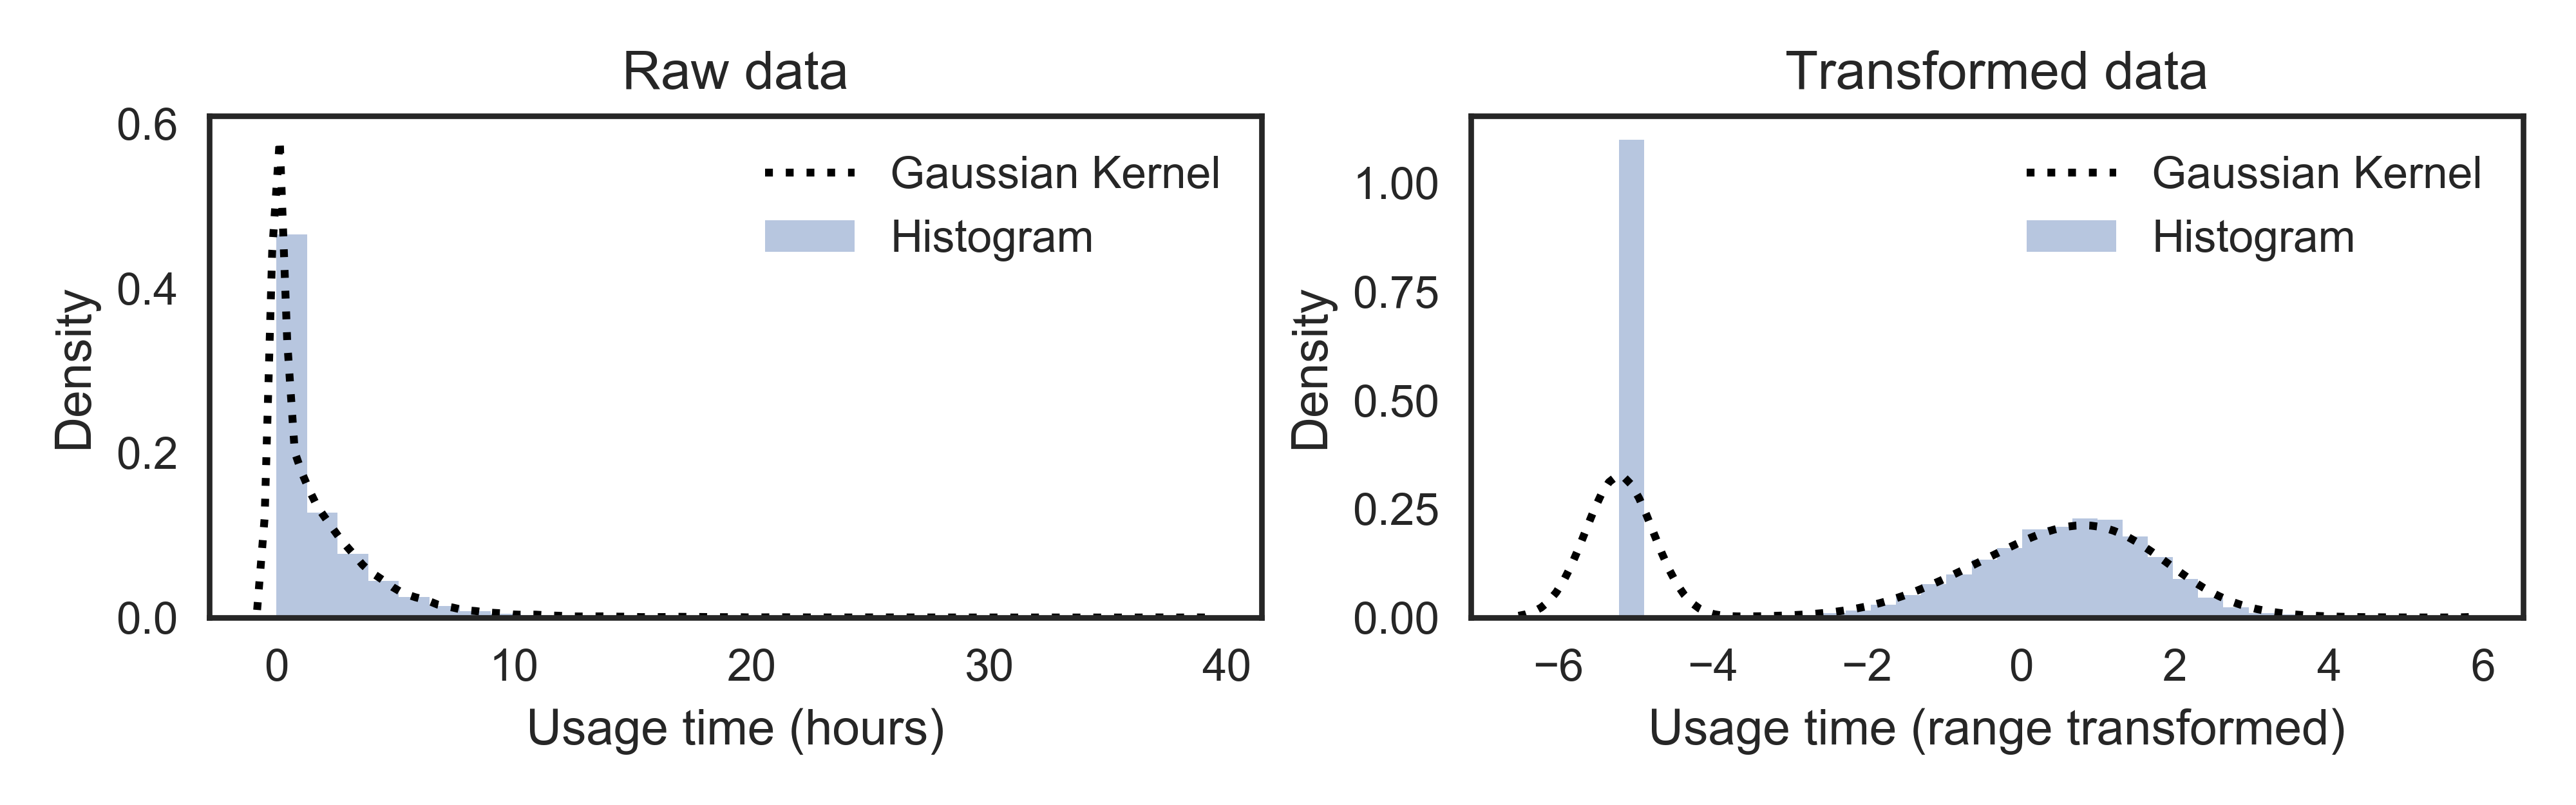
\includegraphics[scale=.7]{BoxCoxTransformation.eps}
\caption{Histograms and Gaussian kernels for raw data and transformed data of feature usage time. We use Box-Cox transformation with $\lambda=0.12$.}
\label{fig:boxcox}
\end{figure}

Standardisation of the data set is also important for our model. The motivation is to scale features into the same range so that the model maintain robustness to very small standard deviations of features. An example is shown in \Cref{fig:dataStandardisation}.

\begin{figure}[!h]
\centering
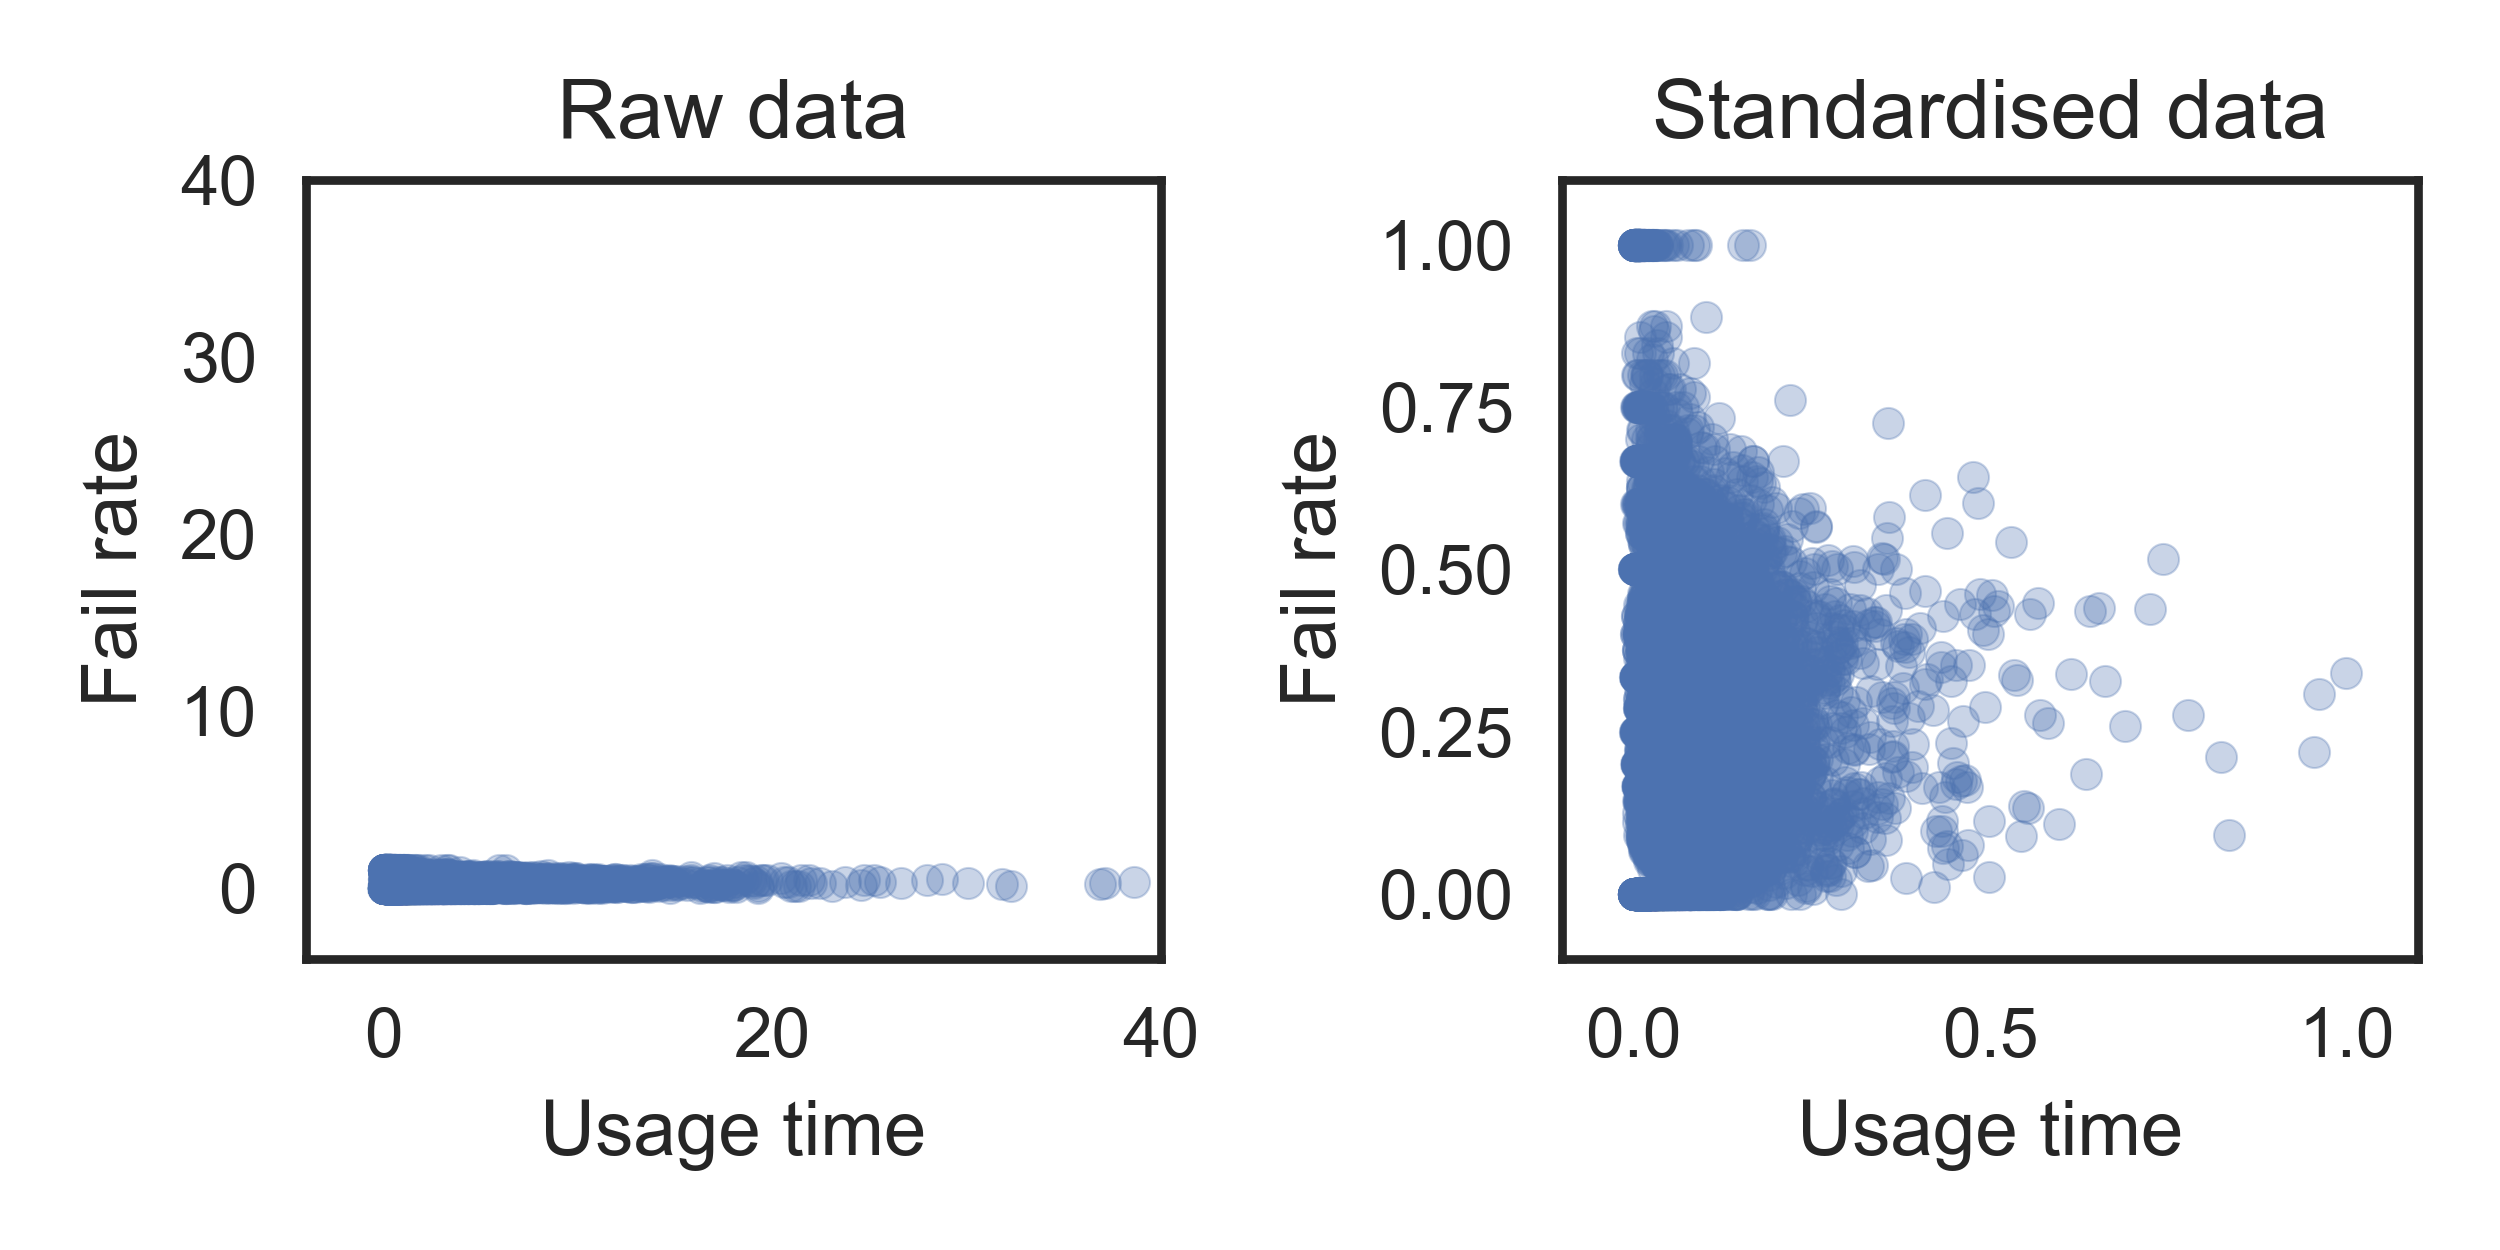
\includegraphics[scale=.7]{DataStandardisation.eps}
\caption{Scatter plot for data of fail rate and usage time. Usage time in hours has a range from 0 to 40 while fail rate only varies from 0 to 1. The variance of fail rate is much smaller than that of usage time. After standardisation, the features have comparable level of values.}
\label{fig:dataStandardisation}
\end{figure}

Formally, we have employed 3 transformations in sequence to make our data more suitable for mixture model learning task. Recall that we denote the feature data by a matrix $\mathbf{X} = (x_{ij}) \in \mathbb{R}^{m \times n}$ (forget about the time subscript as  in (\ref{eq:customerJourney}) for a moment), which describes $n$ observed values for each of the $m$ features. In addition, we denote the $i$-th row of $\mathbf{X}$ by $\mathbf{x}_{i,\text{R}} = [x_{i1} ~x_{i2} ~\cdots ~x_{in}]$. The transformations are performed for each feature separately, resulting in different sets of transformation parameters for different features. To be specific, for $i$-th feature we describe the transformations as following.

\begin{itemize}
\item \textbf{Linear transformation:} The linear transformation is applied either to ensure all data to be positive for eligibility of applying the following power transformation, or to adapt to distributional modelling choice. It has the format:
\begin{equation}
\mathbf{x}_{i,\text{R}}' = a_i \mathbf{1} + b_i \mathbf{x}_{i,\text{R}},
\label{eq:linearTransformation}
\end{equation}
where $a_i$ and $b_i$ are constants and $\mathbf{1} \in \mathbb{R}^{1 \times n}$ is the row vector of all ones.
\item \textbf{Box-Cox power transformation:} The Box-Cox power transformation is used to modify the distributional shape of a set of data to be more normally distributed so that the data appear to more closely meet the assumptions of a statistical inference procedure that is to be applied. It has the format:
\begin{equation}
x_{ij}' = 
\begin{cases}
\frac{x_{ij}^{\lambda_i}-1}{\lambda_i} & \text{if } \lambda_i \neq 0, \\
\ln{x_{ij}} & \text{if } \lambda_i = 0,
\end{cases}
\end{equation}
for $j = 1, ~2, ~\dots, m$. In Box-Cox transformation, $\lambda_i$ is estimated by maximizing the likelihood function \cite{Box64ananalysis}.
\item \textbf{Standardisation:} We choose to scale all features into range $[1, 100]$. If we denote the maximum and minimum values of observed feature $i$ as $x_i^\text{max}$ and $x_i^\text{min}$ respectively, then the standardisation is a linear transformation such that,
\begin{equation}
\mathbf{x}_{i,\text{R}}' = \mathbf{1} + \frac{100-1}{x_i^\text{max}-x_i^\text{min}} \left( \mathbf{x}_{i,\text{R}} - x_i^\text{min} \mathbf{1} \right).
\end{equation}
\end{itemize}

We keep track of all parameters $\{ a_i, b_i, \lambda_i, x_i^\text{min}, x_i^\text{max}\}_{i=1}^m$ involved in the data transformation and standardisation process, because they are needed in prediction task where the feature data for new pupils will be transformed and standardised using the same parameters.